\chapter{Related Work}

In this chapter, we will present several tools with similar focus as our proposed \emph{application generator}. That will help us to identify the key features that we will need to implement in order to achieve our goals. We aim to create a \emph{Linked Data-driven web application generator}. So we have to begin with defining what kind of tools would fall into the same category. Before we start: Let us not limit ourselves only to Linked Data based tools. Firstly, there is not that many similar Linked Data based tools available so there would not be much to analyze. Secondly, we can get interesting findings even from the other tools, as the inner data format is only one aspect of a generator (and for a non-developer, i. e., our potential user, it is definitely not the most important one). We will now move on to the individual features that a tool should have in order to be classified by us as a \emph{data-driven application generator}.

Firstly, such a tool should be a \emph{generator}. That means that whatever the generator produces, it should not disappear after the generator is closed and it should persist as an independent \emph{instance}. This requirement is rather vague as for example any text processor t(e.g. Microsoft Word) would count as a generator in this sense. But it does rule out all kinds of \emph{data viewers}. Secondly, such a tool should generate \emph{applications}. An application, to be called an \emph{application}, should offer (at least potentially) some level of interactivity. For example text documents, images or static visualizations (like non-interactive graphs) are definitely not applications. Lastly, such a tool should be \emph{data-driven}. That means that in a typical scenario, one should start the process with a data set and use this data set to create a new application with the generator.  To give you an example of what we do not consider \emph{data-driven}, we could mention for example the WordPress.com \cite{wordpress} platform. This platform definitely is an \emph{application generator} according to our first two requirements (specifically, it is a \emph{website generator}, or perhaps a \emph{blog generator}). The key difference is that when you create a new application (\emph{website} or \emph{blog}), it is completely empty and then you start adding the data. The process is completely reversed.

We admit that all these definitions are rather vague and it can still be hard to determine whether a certain tool falls into the category of \emph{data-driven application generators}. We believe, however, that all these definitions together give the reader a decent idea of what we consider a \emph{data-driven application generator}.

To make the comparison more organized, we define a limited set of features that we will specifically focus on while examining the tools. An overview table showing the support of these features among all selected tools will be presented to the reader at the end of this chapter. Let us now give a short description of each chosen feature.

\begin{itemize}
\item \emph{Linked Data support}. Our \emph{application generator} is going to be Linked Data based and we consider this aspect one of its biggest assets. Therefore we are naturally interested in the \emph{Linked Data support} of other tools as well.
\item \emph{Extendability}. We want to know whether a particular tool can be programmatically extended to support new types of data and corresponding  new types of applications. By a type of data we do not mean a different format (the data might or might not be represented in RDF, that is irrelevant at this moment) but a different \emph{semantic} meaning of the data. For example, if we decide that our generator should be able to recognize geospatial data and visualize them using an application in the form of a map, can we extend the generator in such a way?
\item \emph{Online sharing}. We want to know whether a generated application can be published online.
\item \emph{Non-developers friendly}. Here we are interested in whether the \emph{application generator} can be operated by a person with no technical knowledge. We are focused specifically on the actual application creation process. An expert might be needed to set up the generator, but this requirement would not break our condition.
\item \emph{Platform}. This feature specifies whether the generator exists in the form of an online \emph{platform} where each user has an account through which he can create, publish and manage his applications.
\item \emph{Configuration}. Here we want to know whether the generator will simply take the input data and generate and publish the application from it, or whether it will offer the user an extra \emph{configuration} step in between, in which the user will be able to affect the final shape of the application before publishing it. This configuration step should allow more than just changing the application name.
\end{itemize}

\def\checkmark{\tikz\fill[scale=0.4](0,.35) -- (.25,0) -- (1,.7) -- (.25,.15) -- cycle;}
\newcolumntype{C}{>{\centering}X} % Create new column type that centers the cell content
\begin{table}[h]
  \caption{Features of related tools}
  \vspace{0.5cm}
  \label{tab:related-features}
\begin{tabularx}
  {\textwidth}{ |r|C|C|C|C|C|C| }
  \hline
      \begin{sideways}Tool\end{sideways} & 
      \begin{sideways}Linked Data support\end{sideways} &
      \begin{sideways}Extendability\end{sideways} &
      \begin{sideways}Online sharing\end{sideways} &
      \begin{sideways}Non-developers friendly\end{sideways} &
      \begin{sideways}Platform\end{sideways} &
      \begin{sideways}Configuration\end{sideways} \tabularnewline \hline
  \hline
% 						&LD			&Extend		&Sharing	&Non-devel	&Platform	&Config	
  Miga Data Viewer		&			& 			&\checkmark &			&			&\checkmark ~ \tabularnewline \hline
  Citadel On The Move	& Y~& Y~& R~& N~& N~& W~ \tabularnewline \hline
  Tableau       		& Y~& Y~& A~& N~& Y~& W~ \tabularnewline \hline
  Avelca                & Y~& N~& - & N~& N~& W~ \tabularnewline \hline  
  Exhibit             	& N~& - & - & N~& - & W~ \tabularnewline \hline
  Payola              	& N~& - & - & N~& - & W~ \tabularnewline \hline
  LinkedPipes           & N~& - & - & N~& - & D~ \tabularnewline \hline

  
\end{tabularx}
\end{table}

\section{Miga Data Viewer}

Miga Data Viewer is a tabular data based \emph{application generator}. It accepts only data formatted in CSV but as this format is widely supported and there is lots of conversion tools available, any source of tabular data (Microsoft Excel file, RDBMC) can be used as an input. Despite the word \emph{viewer} in the name, this tool does meet our requirements to be called an \emph{application generator}. What it generates is an interactive interface that supports browsing, searching and filtering over the input data set. Once it is generated, it can be published online.

\begin{figure}
	\centering
	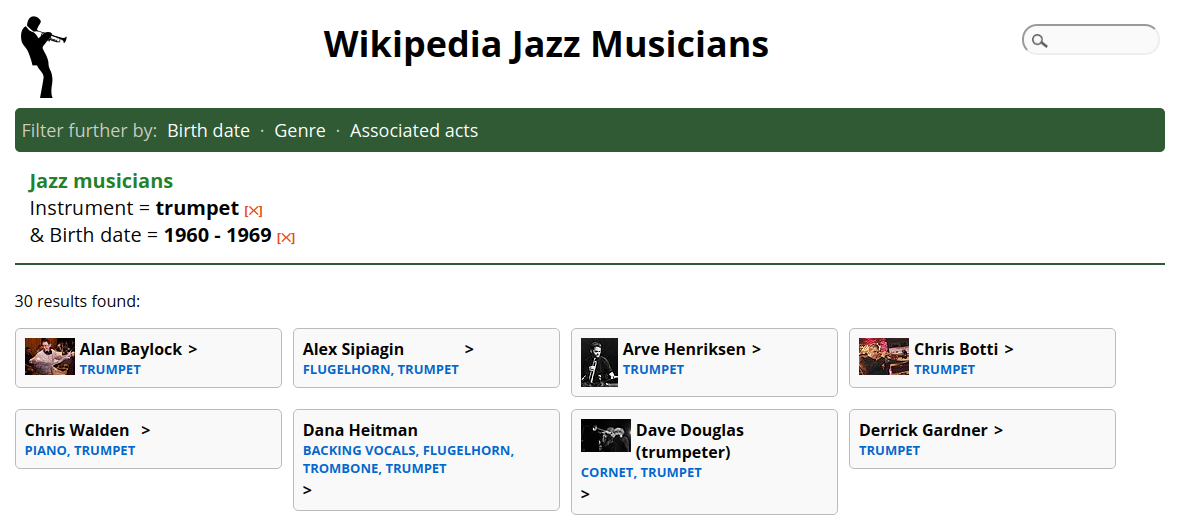
\includegraphics[width=140mm]{img/02_miga_data_viewer.png}
	\caption{Miga Data Viewer: A sample application generated from a set of Jazz Musicians.}
	\label{fig:miga-data-viewer}
\end{figure}

As we already mentioned in the introduction chapter, the big disadvantage of tabular data is that they carry very little semantic information. As without the semantic information, it would be almost impossible to generate anything else but a simple paginated table, the user is required to provide a \emph{schema definition} for each data table (for each single CSV file). That is done through configuration *.ini files using a custom \emph{Miga Data Schema} format. Here is an example of such a configuration:

\scriptsize
\begin{verbatim}
[Books]
Title = Name
Author = List (,) of Entity (Authors/Name)
Number of pages = Number
Genre = List (,) of Text
Wikipedia URL = URL

[Authors]
Name = Name
Birth date = Date
\end{verbatim}
\normalsize

Each section defines a scheme for a CSV file with a name matching the section's name. Each column in the data file is assigned one of the data types provided by the \emph{Miga Data Schema}. Besides the very basic ones (\emph{Text} or \emph{Number} that correspond to data types known from programming languages) and slightly more complex ones (\emph{List} for collections, \emph{Entity} for \emph{foreign keys} as known from relation databases), there are a few special ones with added \emph{semantic meaning}. Let us name for example \emph{URL}, \emph{Image URL} or \emph{Coordinates}. Using these types the Miga Data Viewer is able to create richer interfaces (e.g. it can display entities with coordinates on a map).

It is clear that this format is an attempt of the authors to solve what RDF would be perfect for. But unlike RDF, this format is proprietary so the semantic augmentation will work only with Miga Data Viewer.